\chapter{Related Work and Foundations}\label{sec:related-work}

This Chapter covers terminology, relevant techniques for data visualization and the related work in this area of research.
Advantages and disadvantages of certain data visualization are emphasized.
After introducing visualization techniques, related work on interaction aspects in \cmvs{} is outlined.


\section{Information visualization}
Information visualization is a means of visual communication and has steadily developed since the 16th century~\parencite{Friendly2001}.
It is a generic term, expressing all kinds of effort to put data into visual context to help people understand the significance of data.
Information visualization today goes beyond standard charts and graphs used in spreadsheet applications and covers also infographics, heat maps, geographic visualizations and treemaps~\parencite{Rouse2017}.
Otherwise abstract information is visually represented, making complex data more accessible, understandable and usable.

\textcite{Kusinitz2014} mentions that the human brain processes visual information 60,000 times faster than text and visual content makes up even 93\% of all human communication.
According to the Interaction Design Foundation the purpose of data visualizations is twofold:
Sense-making and communication~\parencite{Few2013}.

Statistical information is abstract and in data visualization ``we must find a way to give form to that which has none.''~\parencite{Few2013}
Successful data visualizations helps the human user to derive knowledge and meta data from the visualization itself.
\textcite{Nocke2002} call this ``visual data mining''.

\section{Data-driven Decision Support Systems}
Data-driven \dss{} are applications to support businesses and organizational decision-making activities in which data visualizations play a key part~\parencite{Nada2007}~\parencite{Poleto2015}.
A common expression by impatient managers who can not afford to wade through lengthy reports has even become the title of a book about \dss{}:
Stephen Few's ``Show me the numbers''.

In the business context, sales managers demand a quick access on the latest data with all relevant visualizations at once.
Examples of this kind of \dss{} are called e.g.\ ``decision cockpit'' or ``business sphere''~\parencite{Davenport2013}.

We can expect to see these technologies more in more in business applications.
\textcite{McAfee2012} from the MIT Center of Digital Business showed that organizations driven most by data-based decision making had 4\% higher productivity rates and 6\% higher profits.

However, little research has been done regarding the performance of \cmvs{} in the field of decision making.
There might be a great potential.
In 1997 \textcite{Mayer1997} conducted eight studies to compare the effect of using multimedia on university students.
The studies showed that when using combined visual and verbal explanations the generation of creative problem solutions increased by an average of more than 50\%.

Apparently, the application of combined data visualization techniques in decision making is a promising strategy.


\section{Geovisualization}
The umbrella term ``Geovisualization'' covers visualization techniques for the ``visual exploration, analysis, synthesis and presentation of geospatial data (any data having geospatial  referencing)''~\parencite{Maceachren2001}.
The entities of geospatial data may include buildings, streets, landmasses, terrain, administrative districts and also moving entities like cars.

\subsection{Visual Variables}\label{sec:related-work:visual-variables}
French cartographer Jaques Bertin introduced seven visual variables in 1967~\parencite{Bertin2010}.
Figure~\ref{fig:related-work:visual-variables} shows these visual variables.
These visual variables are used in cartography but can also be applied to data visualization in general.
\textcite{Carpendale2003} explains in detail their use in computational information instead of printed cartography.
\textcite{Garlandini2009} put these visual variables under systematic validation procedures.
The authors conclude that the variable \attr{size} provides the most accurate and efficient performance while the variable \attr{orientation} provides the least performance.
Bertin's visual variable play a role in interaction aspects of \cmvs{} as they are used to communicate the effect of an interaction.
A highlighted data point can be highlighted by changing the colour or increasing the size of a point.

\begin{figure}
  \centering
  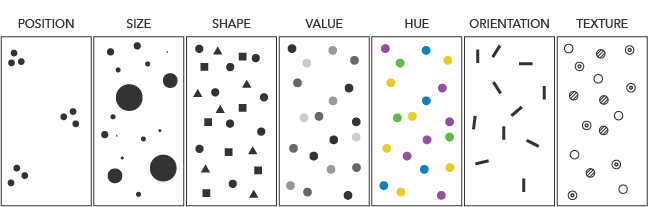
\includegraphics[width=\textwidth]{figures/related-work/visual-variables}
  \caption{Bertin's original visual variables~\parencite{Foster2017}.}
  \label{fig:related-work:visual-variables}
\end{figure}

\subsection{Choropleth maps}
Choropleth maps are thematic maps in which areas are shaded or patterned in proportion to the statistical variables being displayed on the map.
A popular use case is the display of population density or per-capita income.
An example of a choropleth map is shown in Figure~\ref{fig:related-work:choropleth}, visualizing the percentage of obese population in the US\@.
Choropleth maps are very popular and therefore many people are familiar with them already.
A downside of choropleth maps is that larger regions may appear more emphasized than smaller ones, since the entire area of regions is coloured.
Another disadvantage of choropleth maps is the common error of incorrect encoding:
Such an incorrect encoding would be the display of absolute numbers, e.g.\ total population or proceeds of crime, rather than relative numbers, e.g.\ population density or unemployment rate.

\begin{figure}
  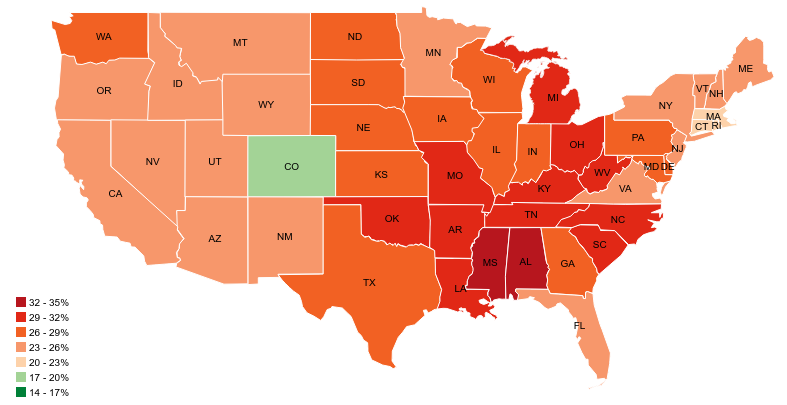
\includegraphics[width=\textwidth]{figures/related-work/choropleth}
  \caption{%
    Choropleth map of obese population, \gls{bmi} $ > 30 $, in the United States in 2008~\parencite{NCCDPHP2017}.
  }\label{fig:related-work:choropleth}
\end{figure}

This work uses a choropleth map for the geographic visualization because of its widespread recognition.

\section{Information Visualization of Hierarchical Data}
The visualization of hierarchical data has a long tradition.
The traditional visual representation of a tree is a directed graph with the root node at the top, as seen in Figure~\ref{fig:related-work:tree-graph}.

An common use case is a directory tree of a file system, e.g.\ a file browser or the command line utility \texttt{tree} on UNIX based operating systems.
As \textcite{Shneiderman1992} mentions, this visualization becomes increasingly large when displaying more than one level and soon exceeds the entire screen size.

\begin{figure}
  \centering
  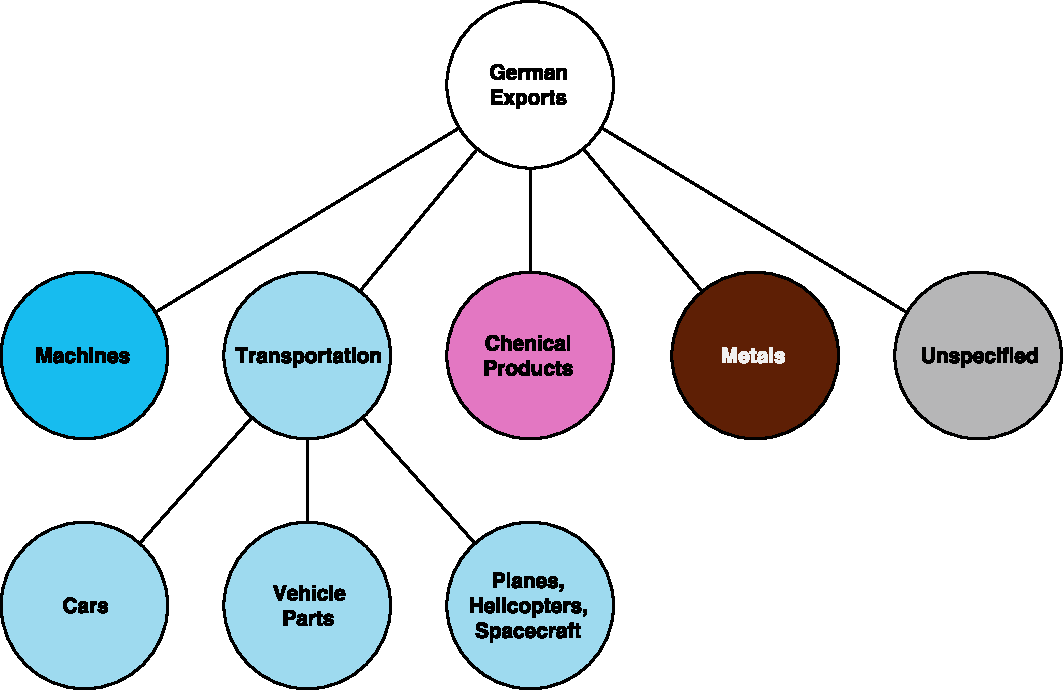
\includegraphics[width=0.6\textwidth]{figures/related-work/Treegraph}
  \caption{
    Traditional visualization of a tree in form of a directed graph with edges and nodes and the root node at the top.
    This example visualizes equivalently a part of the treemap visualization of German exports in Figure~\ref{fig:related-work:treemap-german-exports-1}.
  }
  \label{fig:related-work:tree-graph}
\end{figure}

\subsection{Treemaps}
\textcite{Johnson1991} propose the treemap visualization technique, in which each node is a rectangle whose area is proportional to a specified dimension.
In treemaps every node is visualized as a tile.
The membership relationship is expressed with tiles containing other tiles, thus representing the hierarchy.

Figures~\ref{fig:related-work:treemap-german-exports-1} shows an example of a treemap and Figure~\ref{fig:related-work:treemap-german-exports-2} shows the same treemap in another level of detail.
German exports are divided in generic groups like ``Machines'' and ``Chemical Products'' and include more specific groups like ``Cars'' and ``Packaged Medicaments''.
The user can click on a drop-down menu to change the current level of hierarchy, only leaf nodes are displayed at a time.

The advantage of treemaps is that they are space-filling visualizations, i.e.\ they make 100\% use of the available screen size.
A treemap will, unlike a graph representation of a tree, never exceed the size of the screen.

The area of the tiles can be mapped to a data attribute, e.g.\ the file size on disk or, in cases of Figures~\ref{fig:related-work:treemap-german-exports-1} and~\ref{fig:related-work:treemap-german-exports-2}, the percentage of export quota.
Thus, a treemap can display even more information than a traditional graph representation.
A disadvantage of treemaps is the variable size of each node.
If more and more nodes are displayed, the size of each tile will get smaller and smaller and e.g.\ there might not be enough space to display a label.
You can see this problem occur in Figure~\ref{fig:related-work:treemap-german-exports-2}.

\begin{figure}
    \centering
    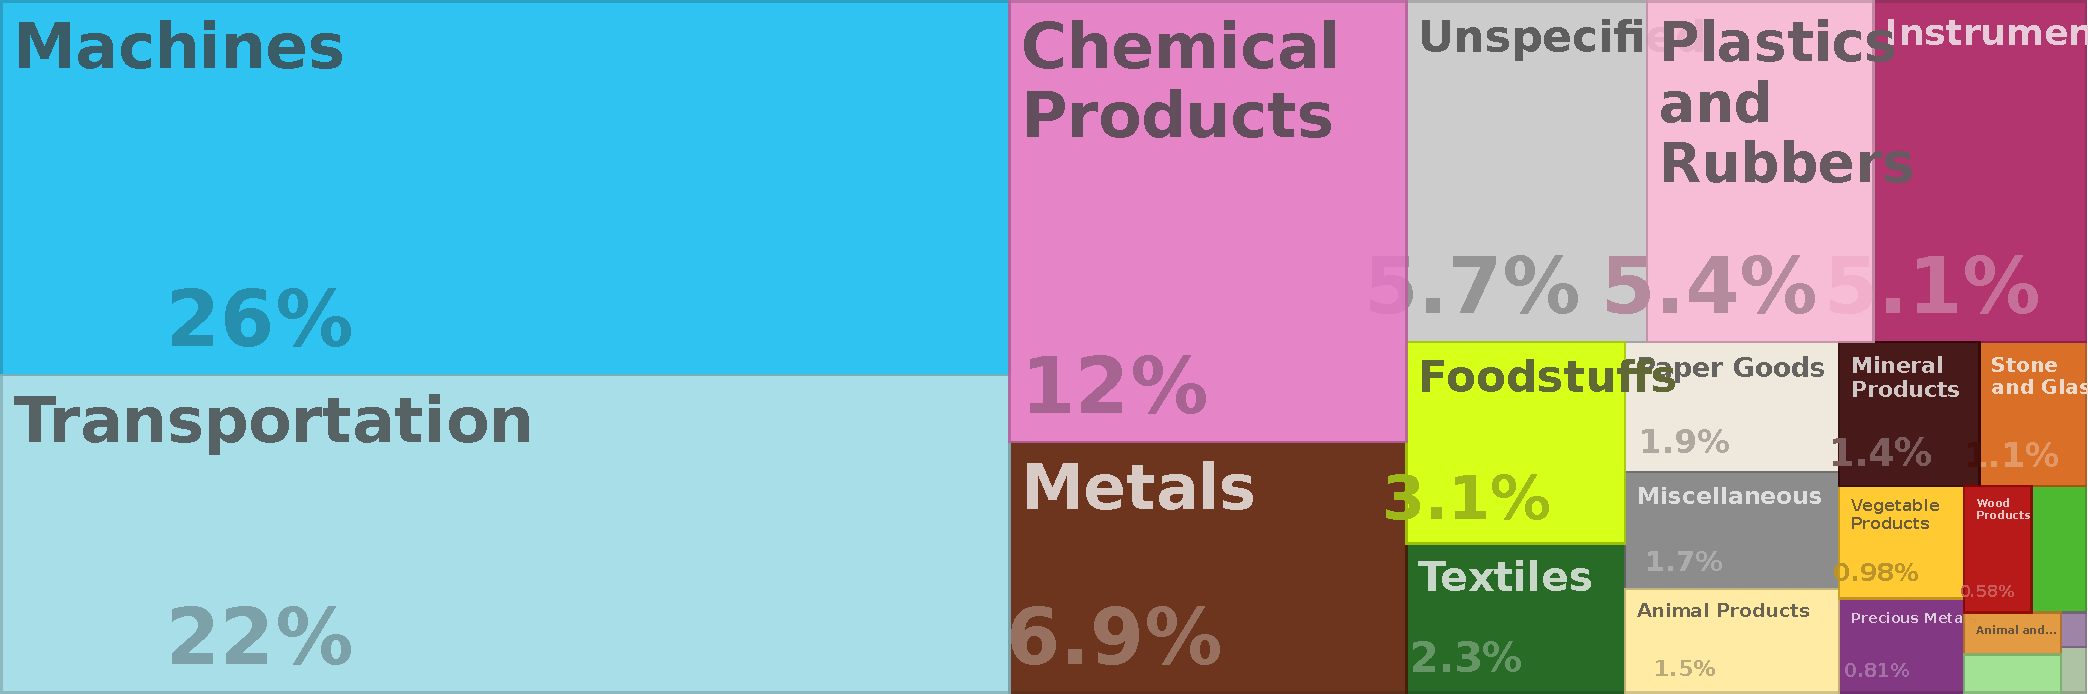
\includegraphics[width=\textwidth]{figures/related-work/en_profile_country_deu_1}
    \caption{A two dimensional treemap of Germany's foreign trade quota of exports, showing only the first hierarchy level~\parencite{Observatory2017}.}
    \label{fig:related-work:treemap-german-exports-1}
\end{figure}

\begin{figure}
    \centering
    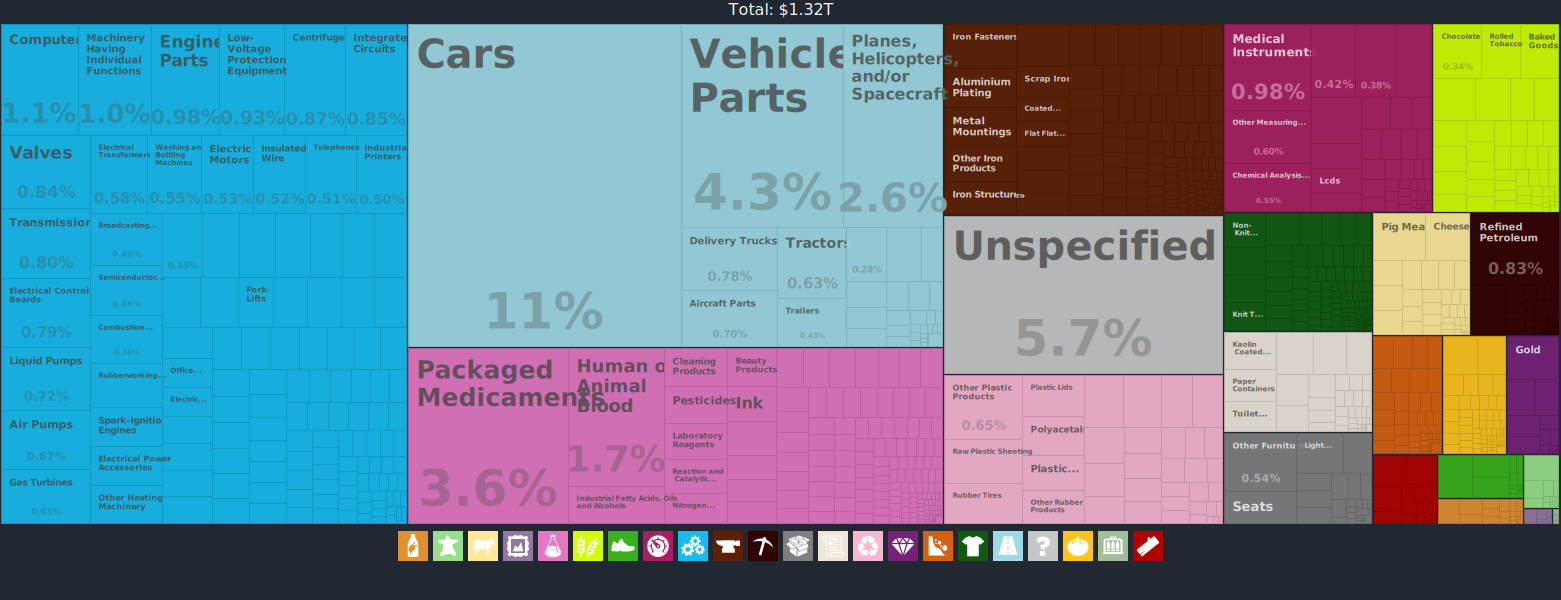
\includegraphics[width=\textwidth]{figures/related-work/en_profile_country_deu_2}
    \caption{Second level of detail of the treemap in Figure~\ref{fig:related-work:treemap-german-exports-1}~\parencite{Observatory2017}.}
    \label{fig:related-work:treemap-german-exports-2}
\end{figure}

If treemaps are used to visualize geographic data like municipalities, real estates or streets, the placement of nodes depends on the tiling algorithm and not the geographic location on a map.
Let's say a treemap visualizes a hierarchy of federal states and municipalities with the area of each tile mapped to the total population of administrative district.
Even if the membership hierarchy is matched by the treemap, the placement of districts in the same hierarchy level is based on their total population and not their geographic location.

\subsection{Spatially Consistent Treemaps}
When visualizing geographical data with a treemap, e.g.\ census data, it is desired to have a spatially consistent visualizations
The layout of hierarchical administrative subdivisions should approximately match a \gv{} of these subdivisions.
An early algorithm for geographically consistent treemaps is called ``Spatially Ordered Treemaps'' by \textcite{Wood2008}.
It is a modification of the ``Squarified Treemap Algorithm''~\parencite{Bruls2000}.
This modification places nodes based on their distance to the enclosing rectangle to be filled, rather than in the weight sequence order.
As \textcite{Ghoniem2015} demonstrate, this algorithm shows undesirable fragmentation for large, flat hierarchies.
One especially serious manifestation of this problem is visible in Figure~\label{fig:related-work:spatially-ordered-treemap}.

Less fragmented but also less consistent regarding the geographic correctness are ``Histomaps'' by \textcite{Keim2002}.
This treemap algorithm sorts nodes such that their direction in the layout approximates their direction with regard to latitude and longitude.
This does not lead to fragmentation, but also does not guarantee geographic correctness.

\textcite{Ghoniem2015} developed ``Weighted Maps'' which are considered to be a trade-off algorithm for ``HistoMaps''.
This trade-off is between aspect ratio and geographic correctness.
Generally speaking, these treemap algorithms suffer because two unrelated circumstances are visualized in the same view.
For that reason, the approach in this paper is to establish the geographic context in a separate view and let treemaps excel in what they are best:
Visualizing hierarchical data.

\begin{figure}
  \centering
  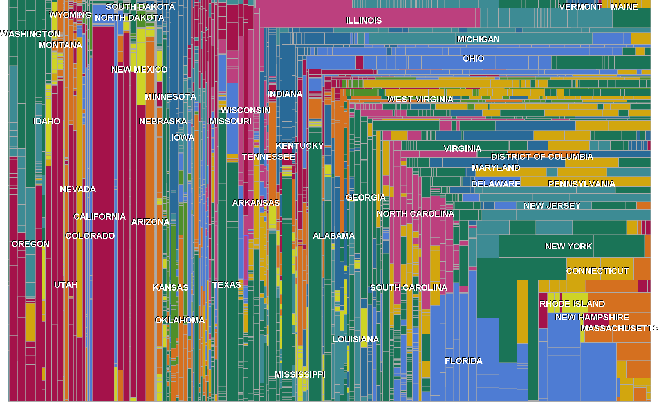
\includegraphics[width=\textwidth]{figures/related-work/spatiallyOrderedTreemap}
  \caption{
    A ``Spatially Ordered Treemap'' by \textcite{Wood2008} visualizing the population in 3,109 counties in the USA~\parencite{Ghoniem2015}.
    This algorithm shows severe fragmentation for large, flat hierarchies.
  }\label{fig:related-work:spatially-ordered-treemap}
\end{figure}


\subsection{3D treemaps and \tmaps{}}
3D treemaps are a concept introduced by \textcite{Bladh2004} in 2004.
The authors transfer the concept of treemaps from two dimensional into three-dimensional space, transforming tiles to blocks.
They introduce ``StepTree''~\parencite{Bladh2004}, which is a three-dimensional treemap to display a directory layout of a file system.
It ``differs from treemaps in that it employs three dimensions by stacking each subdirectory on top of its parent directory.''

3D treemaps are superior to 2D treemaps for tasks with a pronounced topological challenge.
Users perform significantly better in interpreting the hierarchical structure.
However, 3D visualizations also introduce some disadvantages.
Blocks can superimpose each other, forcing the user to navigate the view point.
The navigation of the view point itself is an increase of complexity not present in two dimensional treemaps.

The term \tmap{} was coined by \textcite{Limberger2016} in 2016.
A \tmap{} is just an ordinary 3D treemap, but it has all blocks attached to the ground, or more specifically, attached to the parent block.
An example of a \tmap{} is shown in Figure~\ref{fig:research:ua_treemap}.

\begin{figure}
  \centering
  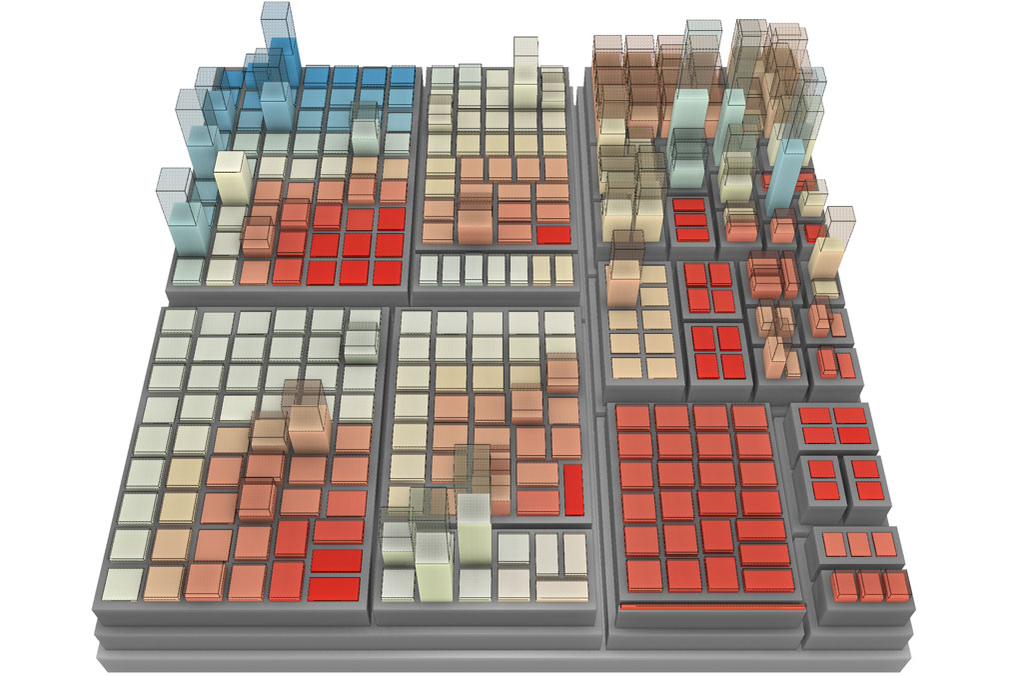
\includegraphics[width=\textwidth]{figures/related-work/2_5D_treemap_example}
  \caption{Example of a \tmap{}~\parencite{Doellner2017}.}
  \label{fig:research:ua_treemap}
\end{figure}

\section{Coordinated Multiple Views}\label{sec:related-work:cmvs}
\cmvs{} are a combination of data visualizations of the same data set in multiple views, often side-by-side.
According to \textcite{Roberts2007} \cmvs{} is just ``a specific exploratory visualization technique that enables users to explore their data''.
Because ``the overall premise for the technique is that users understand their data better if they interact with the presented information and view it through different representations.''~\parencite{Roberts2007}

An example of a \cmv{} is shown in Figure~\ref{fig:related-work:cmv}.
It displays spatial and temporal attributes of pictures from a picture database, as well as continuous attributes like popularity and number of comments.
The user can move the mouse cursor over each item in the scatter plot and the graduated symbol map and the corresponding item is highlighted with a larger stroke in all other views.
On the time line below, the user can also filter for pictures in a certain time frame by dragging the mouse from lower to upper limit.

\begin{figure}
  \centering
  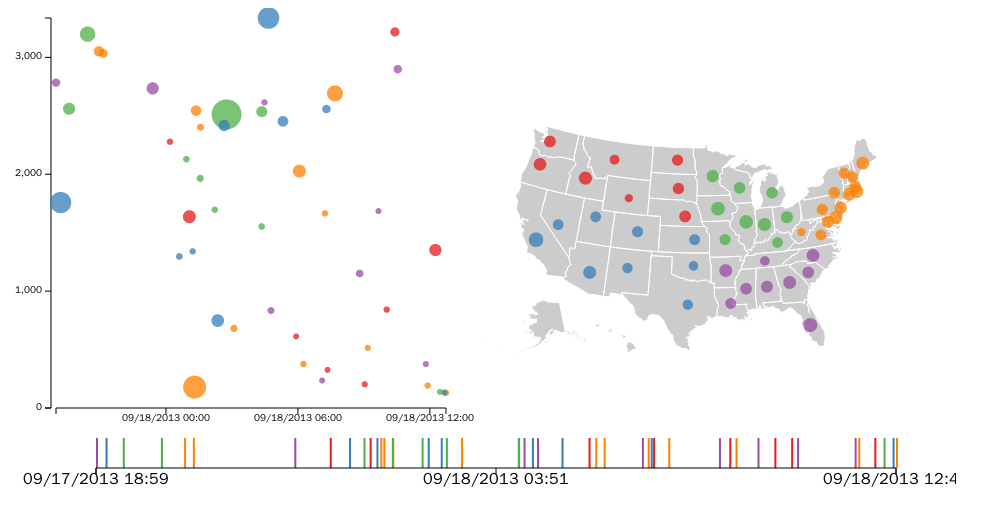
\includegraphics[width=\textwidth]{figures/related-work/cmv}
  \caption{\gls{cmv} displaying the popularity, number of comments, location and time of pictures in a picture data base~\parencite{Dukevis2017}.}
  \label{fig:related-work:cmv}
\end{figure}

\subsection{Brushing and Linking}
Brushing and linking is a common interaction pattern found in \cmvs{} and often a crucial part of these visualizations.
``The technique of brushing is the principle approach, where elements are selected (and highlighted) in one display, concurrently the same information in any other linked display is also highlighted.''~\parencite{Roberts2007}

An example is given in Figure~\ref{fig:research:brushing-linking}.
It displays an on-time performance of airlines, visualized with the ``Crossfilter'' javascript library.

This library is also one of the very few examples of an interaction framework for \cmvs{}.
However, this library is unmaintained as of December 2017, the most recent commit dating back to March 2016.

Each of the flight in the data set has an hour and a date for departure, an arrival delay, which can also be negative, and a traveled distance in miles.
The user can ``brush'' the data by selecting an interval by dragging the mouse.
The respective view will become a primary view and display the deselected items with a grey colour.

All other views become secondary views and display only selected items.
The visualization takes the most recent 80 flights from the database that match all given filters.
The user can further filter for items by dragging another interval in one of the secondary views.

This technique of propagating interactions to other views is called ``linking''.

Figure~\ref{fig:research:brushing-linking} shows a filter for travels with a long delay, i.e.\ from 120 minutes to the maximum value, see the selection in the upper center.
In the view in the upper left corner in Figure~\ref{fig:research:brushing-linking} long delays correlate with the time of the day.

\begin{figure}
  \centering
  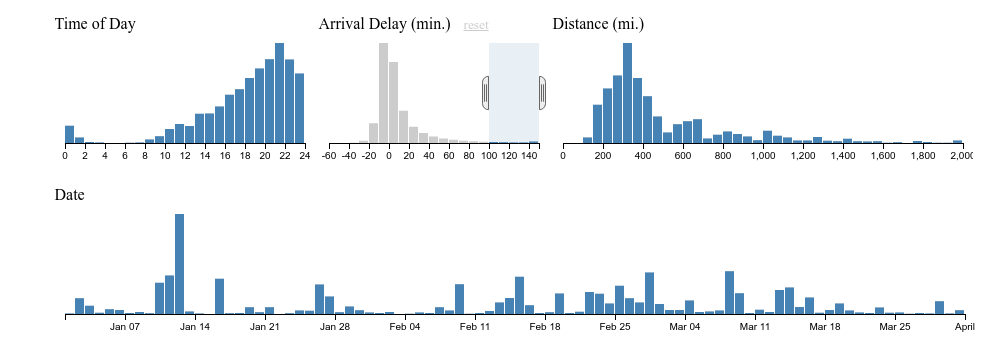
\includegraphics[width=\textwidth]{figures/related-work/brushing_linking}
  \caption{Airline on-time performance: Correlation of time of day with arrival delay. Most recent flight with a delay of more than 100 minutes selected~\parencite{Bostock2017}.}
  \label{fig:research:brushing-linking}
\end{figure}

\section{Technologies}

\todo[inline]{
  This section is a stub, because I guess it will be removed.
  Do we actually need to introduce these technologies in this chapter?
}

\textbf{Leaflet}
Leaflet is the leading open-source JavaScript library for mobile-friendly interactive maps~\parencite{Leaflet2017}.
It has support for GeoJSON which makes it very easy to display tiled web maps with interactive overlays.

\textbf{Web components} is a recent standard of the \textcite{W3C2017} to bring component-based software engineering to the world wide web.
Web components are a set of web platform APIs to create new custom, reusable, encapsulated HTML tags that can be used in web pages and web applications~\parencite{WebComponents2017}.
If \cmvs{} are implemented in JavaScript based web applications, web components are a promising choice, to allow arbitrary views to be put together.

\textbf{GlimmerJS} is the rendering enginge of EmberJS~\parencite{Glimmer2017}.
In 2017 it was released as a standalone component framework.
Applications written in GlimmerJS can be exported as web components.
These web components can be included in any website, which makes GlimmerJS a reasonable choice to build high-quality widgets for user interfaces.
GlimmerJS also uses handlebars~\parencite{Handlebars2017}, a user-friendly templating language.
The downside of GlimmerJS is the current lack of documentation and immaturity due to the recent first release this year.

\textbf{Google Polymer} is another popular library to build web components~\parencite{Polymer2017}.
With 18,469 stars on Github it is the most popular framework for web components at the time of writing.
Polymer has a large community and comprehensive documentation and therefore more suitable than GlimmerJS to build \cmvs{}.

\textbf{ReactJS} is an open-source JavaScript library to build user interfaces and allows to create reusable UI components.
React renders HTML on the client, it changes the page without reloading the page.
The framework corresponds with the View in the Model-View-Controller pattern.
React components are structured hierarchically, with each component having dedicated responsibility.
React is explicitly not implementing web components and is not going to implement web components in the future.
It has, in return, a well-known way of integrating the component framework into a legacy application built with e.g.\ jQuery.
Along with its major advantage of easy integration, it has a striving community, lots of documentation and tutorials and it is well tested.

\textbf{PubSubJS} is a topic-based publish/subscribe library written in JavaScript~\parencite{PubSubJS2017}.
Topics can be registered hierarchically, with subtopics delimited by dots.
A subscription to topic \attr{mcv.select.focus} will be notified only for \attr{focus} interactions whereas a subscription of \attr{mcv.select} will be notified for both \attr{focus} and \attr{highlight} interactions.
Furthermore, topics are published asynchronously, so if the user interacts with a visualization, that does not block code execution.




\section{Interaction Theory}\label{sec:related-work:interaction-theory}
According to \textcite{Ho2013} interactions are a crucial part of data visualizations, yet most research in the area still focuses on visual representations.
Roughly speaking, research on interaction falls into these groups:
How to categorize interaction techniques?
How to find new interaction techniques and apply those to visualizations?

The following sections will give an overview of the current research of interaction aspects for each group.

\section{Interaction Categories}\label{sec:related-work:interaction-theory:categories}
This section covers the larger part of research on interactions in \cmvs{}:
High-level classification and categorization.

In 1996 \textcite{Shneiderman1996} classified interactions into these groups:
\begin{enumerate*}[label=(\arabic*)]
  \item
    Gain an \emph{overview} of the entire collection,
  \item
    \emph{zoom} in on items of interest,
  \item
    select an item or group and get \emph{details} when needed,
  \item
    view \emph{relationships} among items,
  \item
    keep a \emph{history} of actions to support undo,
  \item
    allow \emph{extraction} of sub-collections and of the query parameters.
\end{enumerate*}

Two years later, \textcite{Dix1998} identified these categories:
\begin{enumerate*}[label=(\arabic*)]
  \item
    \emph{Highlight and focus} particular subsets of the data,
  \item
    instead of displaying everything simultaneously \emph{access extra information} by drilling down the data,
  \item
    zoom in and out to give an \emph{overview and context},
  \item
    \emph{change parameters} of the \emph{same representation}, e.g.\ another baseline of a stacked bar chart,
  \item
    \emph{change representation} of the \emph{same data} by switching the chart type,
  \item
    \emph{link representations} to determine the relationship between items.
\end{enumerate*}

In 2002, \textcite{Keim2002} comes up with the following classification:
\begin{enumerate*}[label=(\arabic*)]
  \item
    Dynamic \emph{projection} to show all combination of data attributes mapped to the axis of a diagram,
  \item
    focus on a smaller subsets by \emph{filtering} out parts of the data,
  \item
    \emph{zoom} into a subset of the data and get a higher level of detail,
  \item
     drill-down operations to preserve an overview of the data are called \emph{distortion}
  \item
    and finally \emph{link and brush} visualizations, to highlight the same data points in multiple visualizations.
\end{enumerate*}

The most recent classification was done in 2007 by \textcite{Yi2007} listing seven categories:
\begin{enumerate*}[label=(\arabic*)]
  \item
    \emph{Select} to mark something as interesting,
  \item
    \emph{explore} to show something else,
  \item
    \emph{reconfigure} to show a different arrangement,
  \item
    \emph{encode} to show a different representation,
  \item
    \emph{abstract/elaborate} to show more or less detail,
  \item
    \emph{filter} to show something conditionally,
  \item
    \emph{connect} to show related items.
\end{enumerate*}

It is noticeable that all of these classifications of interactions are redundant.
In this work the classification of \textcite{Yi2007} is used for the remaining parts because it is the most recent classification and it is based on the precursors.

\todo[inline]{Shall I give an example for each category of \textcite{Yi2007} classification?}

\section{Formalization of Interactions}
This section covers the smaller part of research in \cmvs{}, research that is \emph{not} related to a high-level classification of interactions.
Not only interactions in \cmvs{} are considered but any kind of a formalization of interaction that may be used as the starting point for a framework for \cmvs{}.

\textbf{ITlib~\parencite{Figueroa2001}} is an architecture and a framework of interaction techniques for virtual reality applications, designed to be extensible and flexible.
New interaction techniques can easily be added and application specific code is seamlessly integrated.

On a low level an interaction technique ``is modeled as a set of filters connected in a small data flow''~\parencite[p.~2]{Figueroa2001}.
These filters are the smallest process unit in the data flow.
Composed of input and output ports, they communicate with other filters, to receive data input from predecessors and send data output to successors.

The framework specifies and stores the interaction techniques along with its filters, the execution model and the scene in XML documents.
The authors chose XML because it can be parsed easily and they generate code in order to target various virtual reality toolkits and environments.

Even though the system describes interactions in an abstract way, the domain of the framework is clearly the interaction of a human body within a 3D virtual reality.
Certain assumptions are made, including the data model, which is the 3D scene, and human computer interaction devices, like the user's hand or the user's head.

The goal is not to better understand the data, which is the common goal in data visualizations.
In this case, the data model is the 3D scene and the goal is to manipulate the 3D scene.

Most importantly, the framework describes interaction techniques for a single viewpoint but not for coordinated multiple views.

\textbf{A framework for Focus+Context Visualization} by \textcite{Bjork1999} is one of the few formalizations of interactions in data visualizations.

The idea behind the concept of focus and context visualization is to present the object of primary interest in full detail while at the same time giving a overview of the surroundings.

The authors of the paper distinguish first-level and second-level information visualizations:
\subparagraph{Visualizations} referred to as $IV$, are triples of a set $[D]$ of underlying data, a visual representation $V$ and $I$ which is the possible interaction or manipulation.
\begin{equation}
  IV([D], V, I)
\end{equation}
If $I$ affects $[D]$ the underlying data set can be manipulated.
Examples would be changes in a spreadsheet editor, or a change of the start and end date of an appointment in a calendar.

If $V$ is affected by $I$ the user can manipulate $IV$ in order to change the way $[D]$ is represented.
This statement holds e.g.\ for an interaction in which the user increases the visible level of hierarchy in a treemap, which is an \attr{abstract/elaborate} interaction according to \textcite{Yi2007}.
The effect of such an interaction is depicted by the change from Figure~\ref{fig:related-work:treemap-german-exports-1} to Figure~\ref{fig:related-work:treemap-german-exports-2} in Section~\ref{sec:related-work:cmvs}.

\subparagraph{Second-level Visualizations} are information visualizations consecutively applied.
The underlying data set $[D]$ of the previous formula is replaced with some information visualization $IV$, which is compatible with $IV'$.
\begin{equation}
  IV'(IV, V', I')
\end{equation}

Focus+context visualizations are second-level visualizations.
An example given by the authors is the  ``rubbersheet'' visualization, that visually distorts a first-level visualization similar to a magnifier.
Regions of primary interest are distorted to appear magnified, while the remaining regions are minified.

The provided formalizations are a good starting point.
Yet, they only consider interactions in the domain of focus and context visualizations, not in data visualization in general.


